\chapter{Structured Literature Review}
\label{ch:literature}

A structured literature review was conducted to identify how past works
approach static analysis with focus on analysis of multiple versions of a given
software, study of false alarms, and alarms classification. Figure
\ref{fig:structured_review} illustrates the design and application of this
structured literature review. The IEEE International Working Conference on
Source Code Analysis and Manipulation (SCAM)\footnote{\url{ieee-scam.org}} is
known to be one of the most influent conferences for static analysis research
and was selected for this review. While we intended to review one additional
conferece, SCAM provided us with a detailed survey on static analysis alarms
processing, as discussed below, which gave us the necessary background to
perform our research.

\begin{figure}[h]
  \centering
  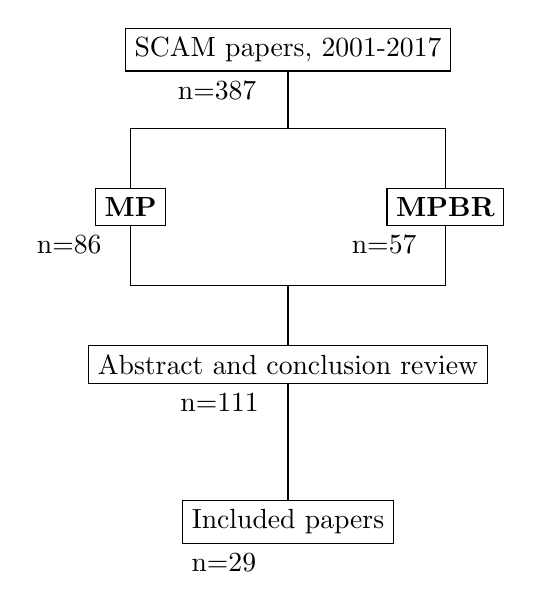
\begin{tikzpicture}[level distance=40mm,sibling distance=5mm]
    \node (1) at (0,0) [draw,label=below left:{n=387}]{SCAM papers, 2001-2017};
    \node (2) at (-2,-2) [draw,label=below left:{n=86}]{\textbf{MP}};
    \node (3) at (2,-2) [draw, label=below left:{n=57}]{\textbf{MPBR}};
    \node (4) at (0,-4) [draw,label=below left:{n=111}]{Abstract and conclusion review};
    \node (5) at (0,-6) [draw,label=below left:{n=29}]{Included papers};

    \draw (node cs:name=1,anchor=south) |- (-2,-1);
    \draw (node cs:name=2,anchor=north) |- (0,-1);

    \draw (node cs:name=1,anchor=south) |- (2,-1);
    \draw (node cs:name=3,anchor=north) |- (0,-1);

    \draw (node cs:name=2,anchor=south) |- (0,-3);
    \draw (node cs:name=3,anchor=south) |- (0,-3);
    \draw (node cs:name=4,anchor=north) |- (0,-3);

    \draw (node cs:name=4,anchor=south) |- (0,-5);
    \draw (node cs:name=5,anchor=north) |- (0,-5);

  \end{tikzpicture}
  \caption{Paper selection}
  \label{fig:structured_review}
\end{figure}


Starting with all SCAM papers published from 2001 (first edition) to 2017,
three search expressions were defined for a first paper selection phase. Since
we are interested in literature related to source code static analysis and  bug
classification to mitigate false positive occurrences, papers containing either
\textit{static analysis}, \textit{false positive} or \textit{bug
classification} were labeled as \textbf{matching papers} (MP).

Then, we defined three categories of interest for a second paper selection
phase. We defined the categories based on the topics related to our research
goal, which, as described in Chapter \ref{cap:introduction}, involves running
multiple static analyzers in different revisions of software to prioritize bugs
and reduce false alarms. The categories defined were:

\begin{itemize}
\item Bug classification
\item Use of multiple static analyzers
\item False alarms in static analysis
\end{itemize}

If a bibliographic reference in any of the papers labeled as \textbf{matching
paper} had a title suggesting that the paper could fit into any of the
categories above, it was labeled as a \textbf{matching paper bibliographic
reference} (MPBR). This inclusion of references was done to select outstanding work in the field,
after noticing common bibliographic references in a significant number of
papers labeled as \textbf{matching papers}.

The abstract and conclusion sections in the papers labeled as either
\textbf{matching papers} or \textbf{matching paper bibliographic references} were read, and the
papers not related to any of the defined categories were discarded.

Finally, all the 36 papers not discarded were selected for this review, as
shown in Figure \ref{fig:structured_review}. In special, Muske and
Serebrenik~\cite{muske2016survey} provided an overview of different techniques
on how to handle static analysis alarms by successfully answering their
research question: \textit{what are possible approaches for handling the static
analysis alarms?} In this survey, the authors classified part of the techniques
as the \textit{automatic post-processing of the alarms}, which includes ranking
or classification of alarms. Given that this survey is strongly related to our
study, we assessed the majority of the survey references under the related
classifications, such as alarms ranking, to better position our work.
Furthermore, other papers, like the ones recommended by the US National
Institute of Standards and Technology (NIST) Software Assurance Metrics And
Tool Evaluation (SAMATE) project
\footnote{\url{samate.nist.gov/index.php/Bibliography.html}} were reviewed as
well ( we did not include them in the structured review numbers).
Appendix\ref{apx:literature} presents a comprehensive list of the papers
reviewed through the methodology here presented.

\section{Related work}
\label{sec:related_work}

Evans~\cite{evans_improving_2002} states that although security vulnerabilities
are well understood, it is not a common practice to include techniques to detect
or avoid them in the development processes and suggests that instead of solely
relying on programmers, tools to prevent and detect software vulnerabilities
should be built and integrated into software development cycles. It is also
known that static analysis helps programmers identify software vulnerabilities
before they reach production~\cite{evans_improving_2002} in a cheaper way than
solely conducting manual inspections~\cite{johnson_why_2013}, thus our interest
in static analyzers.

Several studies propose ways to reduce false positives, which are usually based
on historical analysis~\cite{penta_evolution_2008, spacco_tracking_2006,
kim_which_2007} or some level of statistical analysis~\cite{muske2013review,
boogerd2006prioritizing, kremenek2003z, ruthruff_predicting_2008}. The
remainder of this section discusses related work among the reviewed papers
selected during the structured literature review. First, we define important
terminology that we will use throughout this research. Then, we discuss works
related to static analysis, reduction of false positives in static analysis
reports, and static analysis warnings ranking or classification.

\subsection{Existing data and terminology}
\label{sub:terminology}

The United States Committee on National Security
Systems\footnote{\url{cnss.gov}} (CNSS) defines \textbf{software assurance} as
the \textit{level of confidence that software is free from vulnerabilities [...]
and that the software functions in the intended
manner}~\cite{instruction20034009}. The National Aeronautics and Space
Administration (NASA) defines software assurance as \textit{the planned and
systematic set of activities that ensure that software life cycle processes and
products conform to requirements, standards, and procedures}, which includes
the disciplines of software safety and software verification and
validation~\cite{nasastd8739}. Both these definitions are adopted by the SAMATE
project. We understand that static analysis is useful to aid software safety
and therefore is strongly related to software assurance.

In this research, the same terminology used by
SAMATE~\cite{black_counting_2011} will be used, in the sense that a software
\textit{vulnerability} is a property of a system's security requirements,
design, implementation, or operation that could be triggered, resulting in a
security failure. A vulnerability is the result of one or more
\textit{weaknesses} in software requirements, design, implementation, or
operation. This definition also means that a single weakness may or may not result in a
vulnerability, depending on the software's usage and execution. Whenever we use
\textit{bugs} or \textit{flaws}, we mean weaknesses, and we will usually refer
to them as flaws, as in SAMATE's SATE V Ockham Sound Analysis Criteria
analysis~\cite{black_sate_2016}.

MITRE Corporation\footnote{\url{mitre.org}} maintains the \textit{Common Weakness
Enumeration}~\cite{cwe_page} (CWE), a community-developed dictionary of
software weaknesses types with the support of several organizations, such as Apple,
HP, IBM, and Microsoft. The CWE entries include, among other information, name
and description of the weakness type, behavior of the weakness, description and
consequences of the weakness exploit, and potential mitigation. Examples of
software weaknesses registered as CWEs are buffer overflows, divisions by zero,
and NULL pointer dereferences. Whenever possible, we will try to describe
specific flaws matching them with CWEs. MITRE also maintains a dictionary for
publicly known software vulnerabilities and exposures, the \textit{Common
Vulnerabilities and Exposures}~\cite{cve_page} (CVE), which maps vulnerabilities
in real-world software.

For SAMATE \cite{black_counting_2011}, a \textit{warning} is an issue identified
by a static analyzer that might be a software flaw, and a \textit{report} is
defined as a set of warnings generated by a single run of a static analyzer in
a software corpus. This terminology is important when referring to static
analyzers and their outputs.

\subsection{Handling Static Analysis Warnings}
\label{sub:related_work}

Previous studies show that the most relevant features for training accurate
machine learning models to arbitrate about the positiveness of static analysis
alarms are extracted from properties intrinsic to the analyzed project,
namely the project change history, function and file names, and even the name
of the programmer who introduced the change that triggered the
alarm~\cite{kremenek2004correlation, heckman2009model, jung2005taming,
ruthruff_predicting_2008, yoon2014reducing}. Although these project-specific
features are in great part responsible for the high accuracy of the models
proposed up to now, a model trained on such features cannot be readily used to
query about alarms generated for other projects, hampering the general
availability of the model in automated post-analysis tools, which could
support developers by decreasing the time spent inspecting false alarms.

Boogerd~\cite{boogerd2006prioritizing} presents a warning ranking technique
that uses the probability of a code section being executed to prioritize
warnings. The authors claim that other than using the warnings severity and the
\textit{Z-ranking} technique, they were not aware of any other methods to rank
warnings by the time of their study. Z-ranking~\cite{kremenek2003z} is a
technique to rank warnings using the frequency counts of true and false
positives. It was validated against random ranking algorithms. The
authors of the Z-ranking technique emphasize that a classification system
cannot be perfect since static analysis cannot be perfect itself.
We also use a random ranking algorithm to assess our warnings ranking approach.

Later, Muske~\cite{muske2013review} pointed out the difficulties in reviewing a high
number of warnings and divided the warnings into different categories to identify
redundant warnings and estimate which categories were more prone to hold false
positives. This work also mentioned that if a code is never executed,
warnings pointing at it should have lower review priority.
We divide warnings into categories and use these categories as one of the features
to train the classification model used to rank warnings.

Ruthruff et al.~\cite{ruthruff_predicting_2008} propose a method to maximize
the return on investment of static analyzers to predict if a warning is an
actionable fault, i.e., if it is not a false positive and if a programmer
should fix it. It uses a screening approach for model building that discards
metrics with low predictive power. Among the factors used to predict false
positives, which happened 85\% of the times, are the priority given by the
static analyzer and the file length and indentation, meaning that, differently
from the Z-ranking approach, the authors did run some static analysis in the
code just to extract factors from it. The present study proposes a method to
rank warnings based only on the information provided by the analyses.

In his work, Spacco et al.~\cite{spacco_tracking_2006} implement a technique
to track static analyzers warnings that correspond to the same flaw across
different software versions. This technique would enable the assembly of tool report
deltas, helping developers to focus only on new flaws. Since false positives
are not usually removed from one software version to another, this approach
could help to identify them. By implementing similar techniques to track
warnings across versions in our continuous static analysis tool, we could to
present static analysis reports containing only the warnings introduced in
specific software versions, diminishing the efforts of analyzing tool reports.
These reduced reports might be useful to reduce the number of false positives shown to software
developers since false positives tend to remain across different versions of a
software package. Authors claim that although it seems an easy task, tracking warnings
across software versions is not a trivial problem. Hence, we leave the technique
implementation for future work, as pointed in Chapter~\ref{ch:conclusion}.

Kim et al.~\cite{kim_which_2007} mention the high rates of false positives in
static analysis and claim that sometimes static analyzers prioritize their
warnings inefficiently. Later, they propose a method to prioritize
warnings by searching for bug fixes in the software change history. They then
assume that if a warning from a specific category was removed by a fix, then
all warnings in that category are important. By improving the precision of the
tools used for the study on finding true positives, the authors showed that the
software change history may be important to prioritize warnings.

In another work, Penta et al.~\cite{penta_evolution_2008} performed an analysis
of the evolution of vulnerabilities detected by static analyzers in three
different open source applications: Samba, Squid, and Horde. The authors
analyzed how the number of vulnerabilities varies over time. Since they
analyzed different development versions (not only releases), they could investigate
aspects of the development process, like bug fixing efforts right before a
release. The work aimed to understand how long vulnerabilities tend
to remain in the system by modeling the vulnerabilities decay time with a
statistical distribution and comparing the decay time of different classes of
vulnerabilities.

Our study differs from the ones cited above by assessing static analysis
warnings only with the information present in the warnings themselves, as
discussed during the introduction of this paper
(Chapter~\ref{ch:introduction}).  This difference makes predicting whether a warning is
an actual bug or a false positive harder, since related works emphasize that
the most important characteristics to do this are internal to the analyzed
project. To compensate for this, we use multiple static analyzers to generate
more information and correlate the information provided by them to better
assess the correctness of a given warning.  Since this strategy still might
result in a low-quality classifier, we turn to ensemble techniques to generate
and combine multiple weak classifiers generated this way into a stronger
one~\cite{aima}.

Xypolytos et al.~\cite{xypolytos2017framework} proposed an approach to
prioritize the output of multiple static analyzers by assigning confidence
scores to the tool warnings based on how well each tool handles a specific flaw
category. Although one may compare the authors' approach to the one presented here
since it also assesses the warnings solely based on the information present in the
warnings themselves, the study is in its initial stages and the authors did not
provide statistically significant results.

Next, we introduce the continuous static analysis system developed during this
work, describe its features and discuss the reasons behind the technical
decision taken during the platform development.
